\documentclass{standalone}
\usepackage{tikz}
\usepackage{ctex,siunitx}
\usepackage{tkz-euclide}
\usepackage{amsmath}
\usetikzlibrary{patterns, calc}
\usetikzlibrary {decorations.pathmorphing, decorations.pathreplacing, decorations.shapes,}
\begin{document}
\small
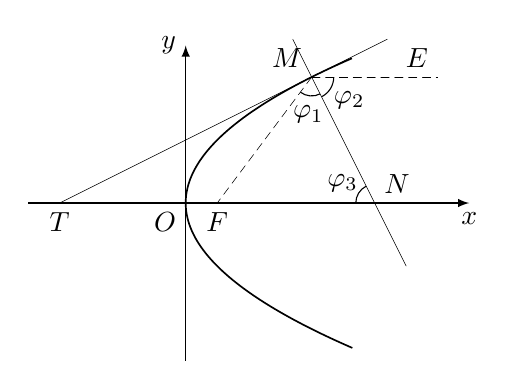
\begin{tikzpicture}[>=latex,scale=0.8]
  \draw[thin,->](-2.5,0)--(4.5,0)node[below]{$x$};
  \draw[thin,->](0,-2.5)--(0,2.5)node[left]{$y$};
  \tkzDefPoints{0/0/O,2/2/M,0.5/0/F,4.0/2/E,-2/0/T,3/0/N}
  \draw[semithick,domain=-2.3:2.3,samples=200] plot({0.5*\x*\x},{\x});
  \tkzDrawSegments[densely dashed](M,E M,F)
  \tkzDrawLine[add = 0.3 and 0.5](M,N)
  \tkzDrawLine[add = 0.3 and 0](M,T)
  \tkzMarkAngle[size=0.3](F,M,N)
  \tkzLabelAngle[pos=0.6](F,M,N){$\varphi_1$}
  \tkzMarkAngle[size=0.35](N,M,E)
  \tkzLabelAngle[pos=0.7](N,M,E){$\varphi_2$}
  \tkzMarkAngle[size=0.3](M,N,F)
  \tkzLabelAngle[pos=0.6](M,N,F){$\varphi_3$}
  \tkzLabelPoints[below left](O)
  \tkzLabelPoints[below](F,T)
  \tkzLabelPoints[above right](N)
  \tkzLabelPoints[above left](M,E)
\end{tikzpicture}
\end{document}